\section{Theory}
Identical infinitely-long metal plates $A_1,A_2,A_3,B_1,B_2,B_3 $ and $B_4$ are placed in an \textit{interleaved} arrangement as dipicted in fig1. Group of plates $A_i$ and $B_i$ are connected to the terminal $A$ and $B$ , respectively, by means of gold wires. which are maintained at constant electric potentials $U_A$ and $U_B$ respectively. \\
Our goal will be to approximate the potential distribution inside the capacitor at steady state with,

\begin{align*}
    &U_A = 5V \\
    &U_B = -5V \\
    &d = 0.5\mu m \\
    &\textit{Dimensions: } 4 \times 4.4 \mu m  
\end{align*}
\begin{figure}[h]
    \centering
    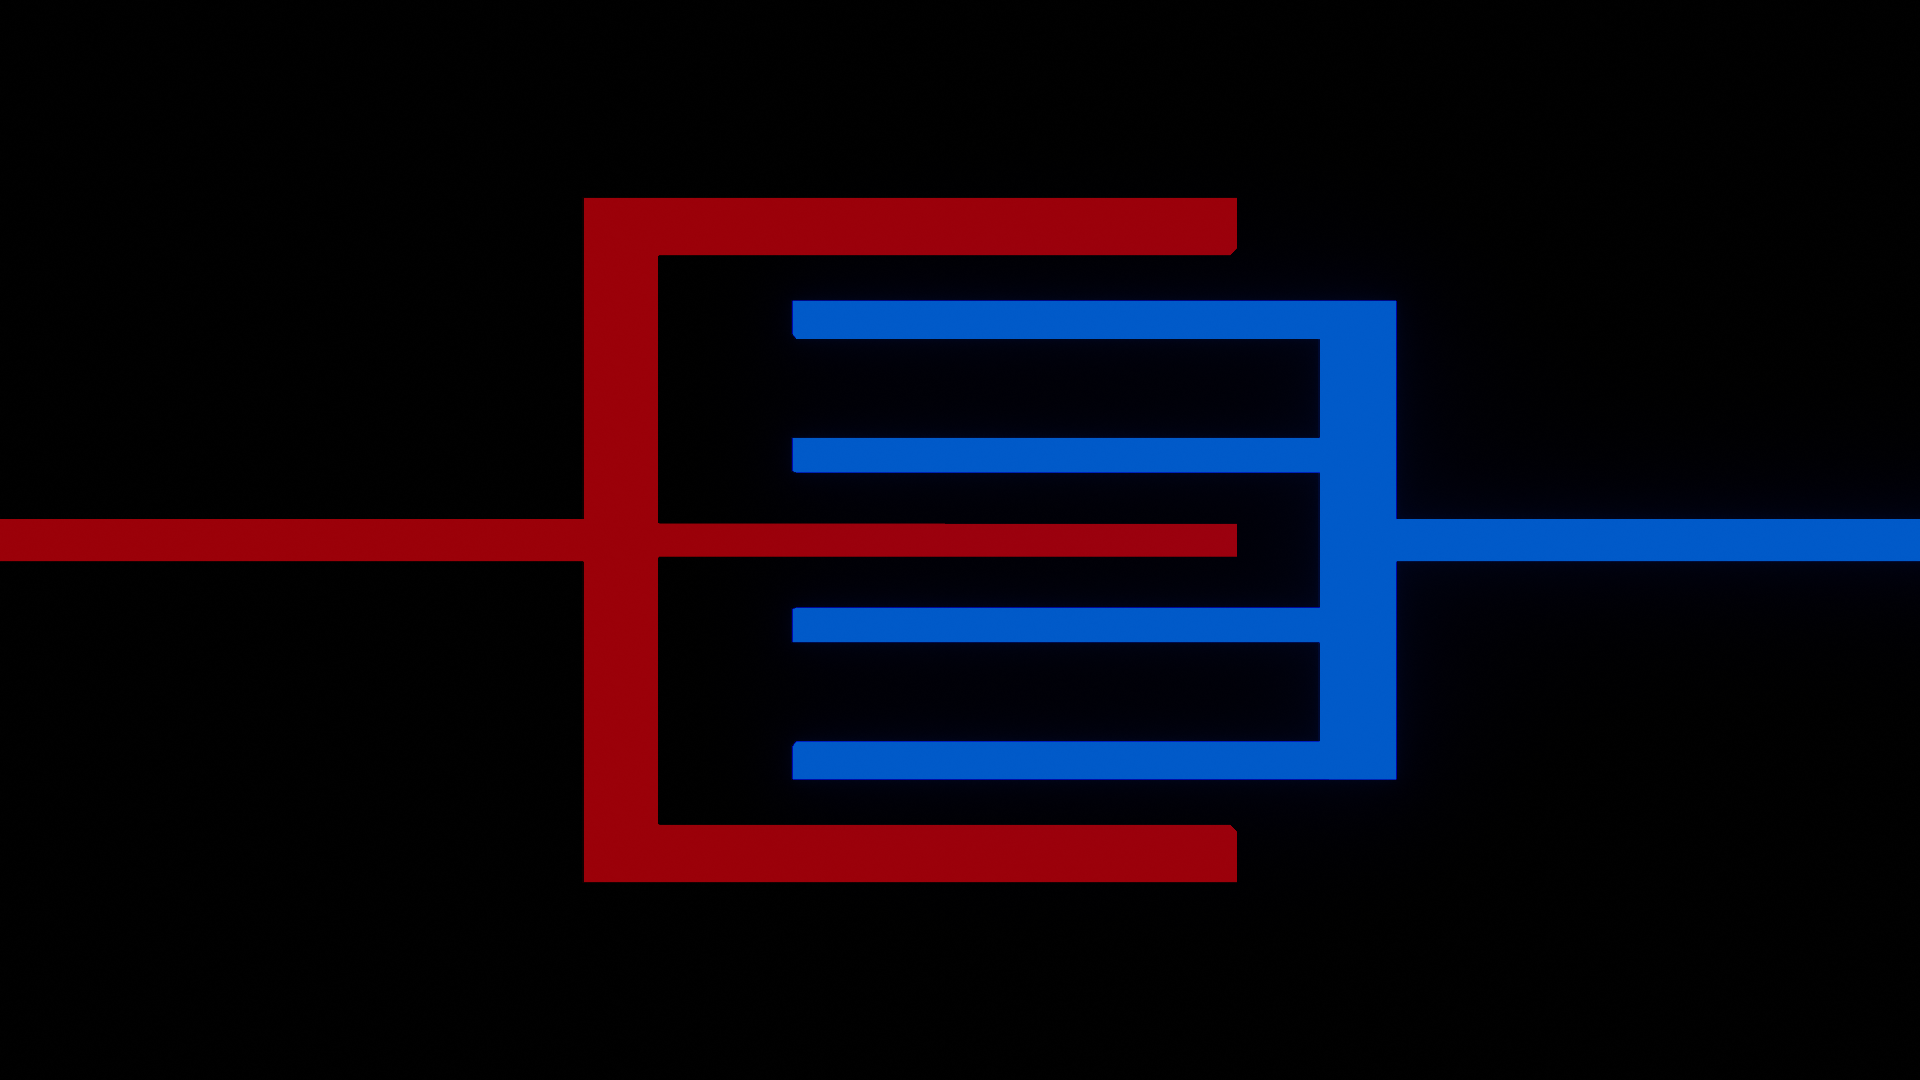
\includegraphics[width=5cm, height=4cm]{content/interleaved_cap_2D.png}
    \caption{\small Diagram dipciting the arrangement of plates in a interleaved fashion.}
    \label{fig 1: the capacitor}
\end{figure}
Mathematical Formulation:

We introduce new variables 
\begin{equation}
    \frac{\pa^2U' }{\pa x^{'2}} + \frac{\pa^2U' }{\pa y^{'2}}= f(x',y') \\
\end{equation}